\chapter{Ứng dụng Alexa}
\ifpdf
    \graphicspath{{Chapter6/Chapter6Figs/PNG/}{Chapter6/Chapter6Figs/PDF/}{Chapter6/Chapter6Figs/}}
\else
    \graphicspath{{Chapter6/Chapter6Figs/EPS/}{Chapter6/Chapter6Figs/}}
\fi

\textit{Nội dung chương 6 sẽ giới thiệu về ứng dụng Alexa, mô hình hoạt động và các thành phần của hệ thống. Chương 6 cũng sẽ giới thiệu về các chức năng của ứng dụng}

\section{Tổng quan}

\section{Mô hình hoạt động}
\begin{figure}[H]
    \centering
    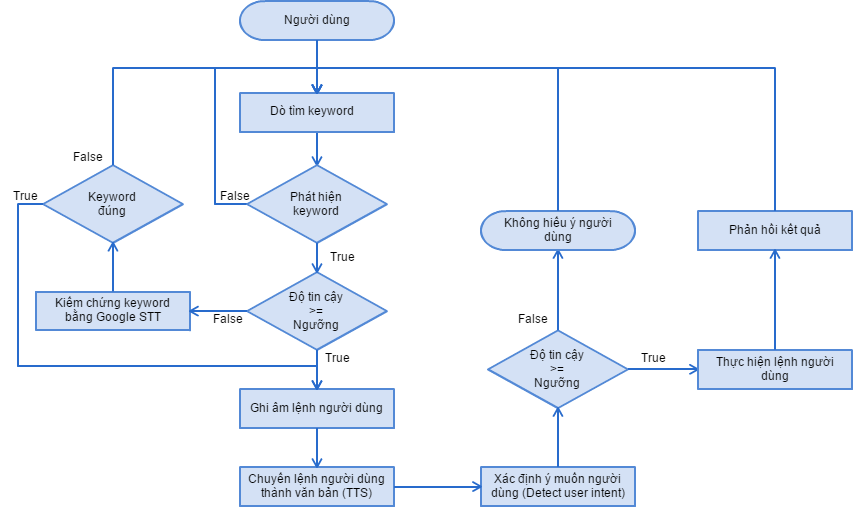
\includegraphics[scale=0.5]{system_flowchart}
    \caption{Mô hình hoạt động của ứng dụng Alexa}
    \label{fig:c6_system_flowchart}
\end{figure}

\subsection{Các module chính}
\subsubsection{Microphone}
\begin{itemize}
\item \textbf{Chức năng}: Microphone đảm nhiệm chức năng thu âm thanh cho toàn bộ ứng dụng. Module này cung cấp dữ liệu âm thanh cho hai module Recorder và Wakeup xử lý.
\begin{figure}[h]
    \centering
    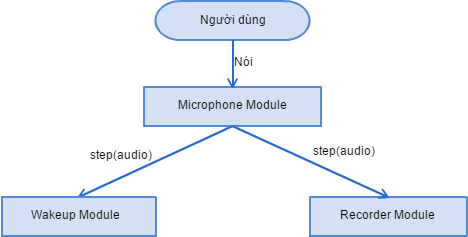
\includegraphics[scale=0.5]{microphone_flowchart}
    \caption{Mô hình hoạt động của module Microphone}
    \label{fig:c6_microphone_flowchart}
\end{figure}

\item \textbf{Cài đặt}: Module Microphone sử dụng thư viện PyAudio để cài đặt và chạy trên một thread riêng biệt với các module khác của ứng dụng.Khi hoạt động module này sẽ đọc dữ liệu audio từ microphone của máy tính và truyền lại cho các module khác sử lý thông qua hàm \lstinline{step(audio)}.

Đoạn code xử lý chính của module Microphone:
\begin{lstlisting}
def run(self):
        if not self.mainControl.isRunning():
            return

        try:
            p = pyaudio.PyAudio()
            self.inputStream = p.open(format=pyaudio.paInt16, channels=cf.paChanels, rate=cf.paRate, input=True, frames_per_buffer=cf.paChunk)
            self.inputStream.start_stream()
        except:
            self.mainControl.onThread(self.mainControl.handleException, self, Microphone.ERR_INPUTSTREAM)
            return

        while True:
            if self.mainControl.isRunning() and self.stopFlag == False:
                buffer = self.inputStream.read(cf.paChunk)
                for listener in self.listeners:
                    listener.onThread(listener.step, buffer) 
            else:
                self.inputStream.stop_stream()
                p.terminate()
                print "Microphone stop"
                break
        self.inputStream.stop_stream()
        self.inputStream.close()
\end{lstlisting}

\item \textbf{API}: Các hàm tương tác mà module Microphone cung cấp
\begin{itemize}
\item \lstinline{addListener(listener)}: thêm đối tượng \lstinline{listener} vào danh sách các đối tượng sẽ nhận được dữ liệu từ microphone.
\item \lstinline{delListener(listener)}: xóa đối tượng \lstinline{listener} khỏi danh sách các đối tượng sẽ nhận được dữ liệu từ microphone.
\item \lstinline{stopThread()}: dừng thread Microphone.
\end{itemize}
\end{itemize}

\subsubsection{Wakeup}
\begin{itemize}
\item \textbf{Chức năng}: Module Wakeup có chức năng dò tìm keyword (trong ứng dụng này keyword là "Alexa"). Mỗi khi người dùng gọi keyword, module Wakeup sẽ phát hiện và chuyển ứng dụng sang trạng thái thu âm để ghi nhận lệnh từ phía người dùng.

\begin{figure}[h]
    \centering
    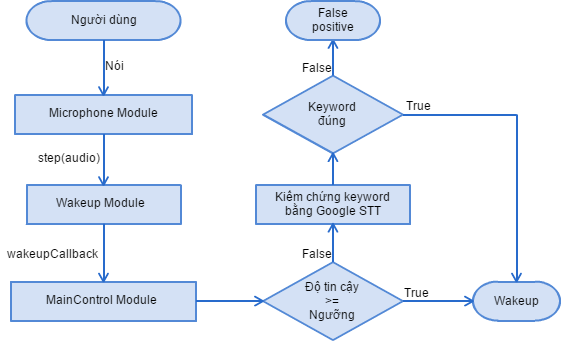
\includegraphics[scale=0.5]{wakeup_flowchart}
    \caption{Mô hình hoạt động của module Wakeup}
    \label{fig:c6_wakeup_flowchart}
\end{figure}

\item \textbf{Cài đặt}: Module Wakeup sử dụng thư viện Pocketsphinx để cài đặt. Module Wakeup sau khi nhận dữ liệu từ module Microphone sẽ gọi hàm \lstinline{process_raw(audio)} của Pocketsphinx để xử lý. Khi Pocketsphinx xác định được keyword, module Wakeup sẽ gửi tín hiệu cho Module MainControl tiếp tục xử lý.

Đoạn code xử lý chính của module Wakeup:
\begin{lstlisting}
def step(self, data):
        self.caches.append(data)

        if self.verify > 0:
            self.verify -= 1

        if self.isPause or rs.isRecording:
            return

        if self.verify % 3 == 1:
            caches_data = b"".join(list(self.caches)) 
            self.mainControl.onThread(self.mainControl.wakeupVerify, caches_data)

        self.decoder.process_raw(data, False, False)
        if self.decoder.hyp() != None:
            for seg in self.decoder.seg():
                if seg.prob >= cf.cmuProbThreshole:     
                    self.mainControl.onThread(self.mainControl.wakeupCallback, seg.word, seg.prob)
                else:
                    self.verify = 5
                    caches_data = b"".join(list(self.caches)) 
                    self.mainControl.onThread(self.mainControl.wakeupVerify, caches_data)
            self.decoder.end_utt()
            self.decoder.start_utt()
\end{lstlisting}

\item \textbf{API}: Các hàm tương tác mà module Wakeup cung cấp
\begin{itemize}
\item \lstinline{step(audio)}: nhận dữ liệu audio và xử lý.
\item \lstinline{pause()}: tạm dừng hoạt động.
\item \lstinline{resume()}: tiếp tục hoạt động.
\item \lstinline{stopThread()}: dừng thread Wakeup.
\end{itemize}
\end{itemize}

\subsubsection{Recorder}
\begin{itemize}
\item \textbf{Chức năng}: Module Recorder có chức năng ghi âm lệnh người dùng. Sau khi người dùng gọi keyword, module Recorder sẽ bắt đầu ghi âm và tự động dừng ghi ăm khi người dùng kết thúc lệnh.

\begin{figure}[h]
    \centering
    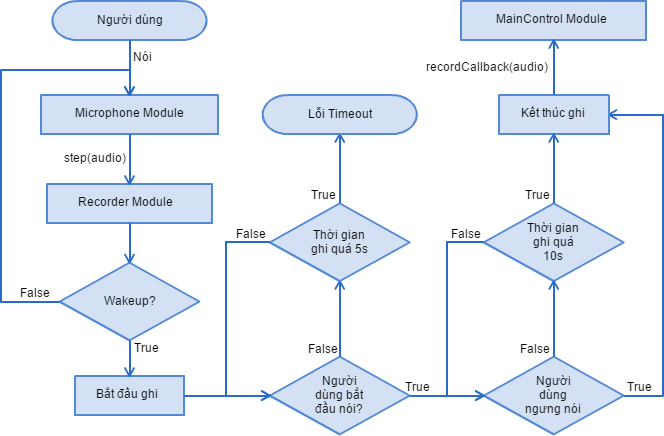
\includegraphics[scale=0.5]{recorder_flowchart}
    \caption{Mô hình hoạt động của module Recorder}
    \label{fig:c6_recorder_flowchart}
\end{figure}

\item \textbf{Cài đặt}: Module Recorder được cài đặt dựa trên mã nguồn của thư viện Google Speech to Text. Module Recorder sau khi nhận dữ liệu âm thanh từ module Microphone sẽ tính giá trị năng lượng của âm thanh (giá trị rms). Dựa vào giá trị năng lượng ta sẽ xác định được thời điểm người dùng bắt đầu nói và ngừng nói. Sau khi kết thúc ghi âm, đoạn âm thanh thu được sẽ được chuyển cho Module MainControl để tiếp tục xử lý.

Đoạn code xử lý chính của module Recoder:
\begin{lstlisting}
def step(self, buffer):
        if self.adjustAmbientNoise and not rs.isRecording:
            energy = audioop.rms(buffer, 2) # energy of the audio signal
            # dynamically adjust the energy threshold using assymmetric weighted average
            damping = self.dynamicEnergyAdjustmentDamping ** self.secondsPerBuffer # account for different chunk sizes and rates
            target_energy = energy * self.dynamicEnergyRatio
            self.energyThreshold = self.energyThreshold * damping + target_energy * (1 - damping)
            return

        # store audio input until the phrase starts
        if not self.isSpeaking:
            self.elapsedTime += self.secondsPerBuffer
            if self.elapsedTime >= cf.rcTimeout: # handle timeout if specified
                self.mainControl.onThread(self.mainControl.handleException, self, Recorder.ERR_TIMEOUT)
                rs.isRecording = False
                return

            self.frames.append(buffer)
            if len(self.frames) > self.nonSpeakingBufferCount: # ensure we only keep the needed amount of non-speaking buffers
                self.frames.popleft()

            # detect whether speaking has started on audio input
            energy = audioop.rms(buffer, 2) # energy of the audio signal
            if energy > self.energyThreshold:
                self.isSpeaking = True
                return

            # dynamically adjust the energy threshold using assymmetric weighted average
            if self.dynamicEnergyThreshold:
                damping = self.dynamicEnergyAdjustmentDamping ** self.secondsPerBuffer # account for different chunk sizes and rates
                target_energy = energy * self.dynamicEnergyRatio
                self.energyThreshold = self.energyThreshold * damping + target_energy * (1 - damping)

        else:
            self.elapsedTime += self.secondsPerBuffer

            self.frames.append(buffer)
            self.phraseCount += 1

            if self.elapsedTime >= cf.rcMaxDuration:
                self.finishRecord()
                return

            # check if speaking has stopped for longer than the pause threshold on the audio input
            energy = audioop.rms(buffer, 2) # energy of the audio signal
            # print "begin speak: " + str(energy) + " - " + str(self.energyThreshold)
            if energy > self.energyThreshold:
                self.pauseCount = 0
            else:
                self.pauseCount += 1

            if self.pauseCount > self.pauseBufferCount: # end of the phrase
                # check how long the detected phrase is, and retry listening if the phrase is too short
                self.phraseCount -= self.pauseCount
                if self.phraseCount < self.phraseBufferCount:
                    # self.mainControl.onThread(self.mainControl.handleException, self, Recorder.ERR_PHRASE_TOO_SHORT)
                    return

                for i in range(self.pauseCount - self.nonSpeakingBufferCount):
                     self.frames.pop() # remove extra non-speaking frames at the end
                self.finishRecord()
\end{lstlisting}

\item \textbf{API}: Các hàm tương tác mà module Recorder cung cấp
\begin{itemize}
\item \lstinline{step(audio)}: nhận dữ liệu audio và xử lý.
\item \lstinline{record()}: bắt đầu ghi âm.
\item \lstinline{finishRecord()}: dừng việc ghi âm và gửi đoạn âm thanh thu được tới MainControl.
\item \lstinline{stopThread()}: dừng thread Recorder.
\end{itemize}
\end{itemize}

\subsubsection{Text To Speech}
\begin{itemize}
\item \textbf{Chức năng}: Module Text to Speech có chức năng chuyển đổi văn bản thành giọng nói để phản hổi cho người dùng.

\begin{figure}[h]
    \centering
    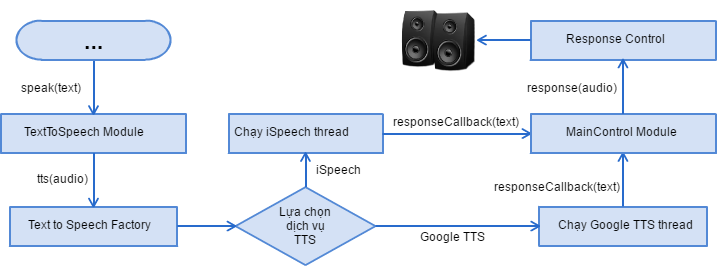
\includegraphics[scale=0.5]{tts_flowchart}
    \caption{Mô hình hoạt động của module Text to Speech}
    \label{fig:c6_tts_flowchart}
\end{figure}

\item \textbf{Cài đặt}: Module Text to Speech (TTS) được cài đặt theo mẫu thiết kế Singleton và Factory. Nhờ mẫu Singleton module TTS có thể được sử dụng từ bất cứ module nào của hệ thống mà không làm phung phí tài nguyên khi phải tạo ra nhiều instance. Mẫu Factory cung cấp quyền lựa chọn dịch vụ TTS, hiện module TTS hỗ trợ hai dịch vụ đó là iSpeech và Google Text to Speech. Sau khi thực hiện xong công việc, tập tin âm thanh thu được sẽ được chuyển cho module MainControl để tiếp tục xử lý.

Đoạn code xử lý chính của module Text to Speech:
\begin{lstlisting}
class TextToSpeech:
    instance = None
    @staticmethod
    def getInstance(callback = None):
        if TextToSpeech.instance is None:
            TextToSpeech.instance = TextToSpeech(callback)
        return TextToSpeech.instance
    
    def __init__(self, callback):
        self.callback = callback
        self.ttsFactory = TTSFacroty.getInstance()

    def speak(self, text):
        if rs.isMute:
            return
        ttsSource = self.ttsFactory.getTTSSource(cf.ttsSource)
        ttsSource.textToSpeech(text, self.callback, self.callback.responseCallback)
        ttsSource.start()

    def play(self, filename):
        if rs.isMute:
            return
        info = {}
        info['url'] = filename
        info['type'] = "tts"
        info['tts'] = "file"
        if self.callback is not None and self.callback.responseCallback is not None:
            self.callback.onThread(self.callback.responseCallback, info)
\end{lstlisting}

\item \textbf{API}: Các hàm tương tác mà module Text to Speech cung cấp
\begin{itemize}
\item \lstinline{speak(text)}: chuyển đổi văn bản \lstinline{text} thành tiếng nói.
\item \lstinline{play(filename)}: phát tập tin âm thanh có đường dẫn \lstinline{filename}.
\end{itemize}
\end{itemize}
\subsubsection{Speech to Text}
\begin{itemize}
\item \textbf{Chức năng}: Module Speech to Text (STT) có chức năng chuyển dữ liệu âm thanh tiếng nói về dạng văn bản. Cụ thể, module này đảm nhiệm hai chức năng chính: chuyển mệnh lệnh của người dùng về văn bản và kiểm chứng lại keyword khi kích hoạt hệ thống.

\begin{figure}[h]
    \centering
    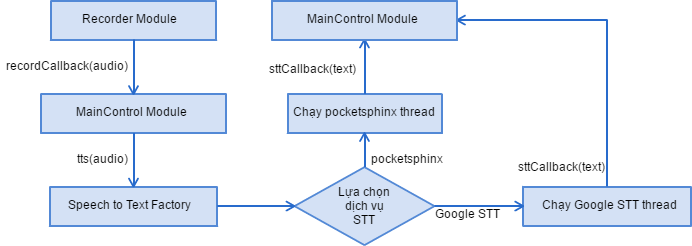
\includegraphics[scale=0.5]{stt_flowchart}
    \caption{Mô hình hoạt động của module Speech to Text}
    \label{fig:c6_stt_flowchart}
\end{figure}

\item \textbf{Cài đặt}: Module Speech to text (STT) được cài đặt theo mẫu thiết kế Singleton và Factory. Nhờ mẫu Singleton module STT có thể được sử dụng từ bất cứ module nào của hệ thống mà không làm phung phí tài nguyên khi phải tạo ra nhiều instance. Mẫu Factory cung cấp quyền lựa chọn dịch vụ STT, hiện module STT hỗ trợ hai dịch vụ đó là pocketsphinx và Google Speech to Text. Sau khi thực hiện xong công việc, đoạn văn bản thu được sẽ được chuyển cho module MainControl để tiếp tục xử lý.

Đoạn code xử lý chính của module Speech to Text:
\begin{lstlisting}
class STTFactory:
    instance = None
    def __init__(self):
        self.map = {}
        self.addSTTSource("googlestt", GoogleSTT())
        self.addSTTSource("sphinxstt", SphinxSTT())
        
    @staticmethod
    def getInstance():
        if STTFactory.instance is None:
            STTFactory.instance = STTFactory()
        return STTFactory.instance
    
    def getText(self, audio, callback, callbackFuncion):
        stt = self.getSTTSource(cf.sttSource)
        if stt is not None:
            stt.setAudio(audio, callback, callbackFuncion)
            stt.start()

    def addSTTSource(self, key, ttsObject):
        self.map[key] = ttsObject

    def getSTTSource(self, key):
        if key in self.map:
            return self.map[key].clone()
        return None
\end{lstlisting}

\item \textbf{API}: Các hàm tương tác mà module Speech to Text cung cấp
\begin{itemize}
\item \lstinline{setAudio(audio)}: nhận dữ liệu audio và chuyển thành văn bản.
\end{itemize}
\end{itemize}

\subsubsection{Intent Detector}
\begin{itemize}
\item \textbf{Chức năng}: Module Intent Detector có chức năng xác định mệnh lệnh của người dùng.

\begin{figure}[h]
    \centering
    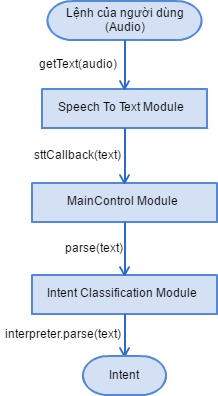
\includegraphics[scale=0.6]{intent_classification_flowchart}
    \caption{Mô hình hoạt động của module Intent Detector}
    \label{fig:c6_intent_classification_flowchart}
\end{figure}

\item \textbf{Cài đặt}: Module Intent Detector sử dụng thư viện Rasa\_NLU để cài đặt. Module Intent Detector sau khi nhận đoạn văn bản của lệnh người dụng từ module MainControl sẽ gọi hàm \lstinline{pasrse(text)} để xử lý. Khi xác định được mệnh lệnh của người dùng, mệnh lệnh này sẽ được chuyển qua cho Module Intent Processor để xử lý.

Đoạn code xử lý chính của module Intent Detector:
\begin{lstlisting}
class IntentDetector:
    instance = None

    @staticmethod
    def getInstance():
        if IntentDetector.instance is None:
            IntentDetector.instance = IntentDetector()
        return IntentDetector.instance

    def __init__(self):
        print "Init Intent Detector"
        metadata = Metadata.load(cf.idModelDir)
        self.interpreter = Interpreter.load(metadata, RasaNLUConfig(cf.idConfigDir))

    def parse(self, text):
        return self.interpreter.parse(text)
\end{lstlisting}

\item \textbf{API}: Các hàm tương tác mà module Intent Detector cung cấp
\begin{itemize}
\item \lstinline{parse(text)}: xác định mệnh lệnh người dùng từ đoạn văn bản \lstinline{text}.
\end{itemize}

\item \textbf{Tập dữ liệu huấn luyện}: Tập dữ liệu huấn luyện cho model Rasa NLU dùng trong hệ thống này gồm 650 mẫu dữ liệu thuộc 31 lớp intent. Có 5 lớp entity khác nhau trong tập dữ liệu.

\begin{longtable}{ |l|l|l|l| }
\caption{Danh sách các intent trong tập dữ liệu huấn luyện}\label{c6_intent_details} \\
\hline
\textbf{Nhóm intent} & \textbf{Intent} & \textbf{Các entity} & \textbf{Số mẫu} \\ \hline
general\_question & general\_question & Không có & 25 \\ \hline
\multirow{6}{*}{music} & music.play & song, artist & 17 \\ \cline{2-4}
& music.stop & Không có & 5 \\ \cline{2-4}
& music.pause & Không có & 4 \\ \cline{2-4}
& music.resume & Không có & 7 \\ \cline{2-4}
& music.forward & Không có & 7 \\ \cline{2-4}
& music.backward & Không có & 7 \\ \hline
\multirow{16}{*}{smalltalk} & smalltalk.agent.acquaintance & Không có & 18 \\ \cline{2-4}
& smalltalk.agent.age & Không có & 8 \\ \cline{2-4}
& smalltalk.agent.birth\_date & Không có & 7 \\ \cline{2-4}
& smalltalk.agent.boss & Không có & 7 \\ \cline{2-4}
& smalltalk.agent.hobby & Không có & 7 \\ \cline{2-4}
& smalltalk.agent.name & Không có & 6 \\ \cline{2-4}
& smalltalk.agent.residence & Không có & 23 \\ \cline{2-4}
& smalltalk.appraisal.good & Không có & 119 \\ \cline{2-4}
& smalltalk.appraisal.thank\_you & Không có & 32 \\ \cline{2-4}
& smalltalk.appraisal.well\_done & Không có & 9 \\ \cline{2-4}
& smalltalk.greetings.bye & Không có & 34 \\ \cline{2-4}
& smalltalk.greetings.goodevening & Không có & 6 \\ \cline{2-4}
& smalltalk.greetings.goodmorning & Không có & 13 \\ \cline{2-4}
& smalltalk.greetings.goodnight & Không có & 19 \\ \cline{2-4}
& smalltalk.greetings.hello & Không có & 18 \\ \cline{2-4}
& smalltalk.user.will\_be\_back & Không có & 5 \\ \hline
time & time.get & location & 91 \\ \hline
\multirow{6}{*}{volume} & volume.check & Không có & 7 \\ \cline{2-4}
& volume.set & number & 10 \\ \cline{2-4}
& volume.up & number & 12 \\ \cline{2-4}
& volume.down & number & 17 \\ \cline{2-4}
& volume.mute & Không có & 9 \\ \cline{2-4}
& volume.unmute & Không có & 7 \\ \hline
weather & weather.get & Không có & 94 \\ \hline
\end{longtable}
\end{itemize}

\subsubsection{Intent Processor}
\begin{itemize}
\item \textbf{Chức năng}: Module Intent Processor có chức năng xử lý và trả về kết quả của mệnh lệnh từ người dùng.

\begin{figure}[h]
    \centering
    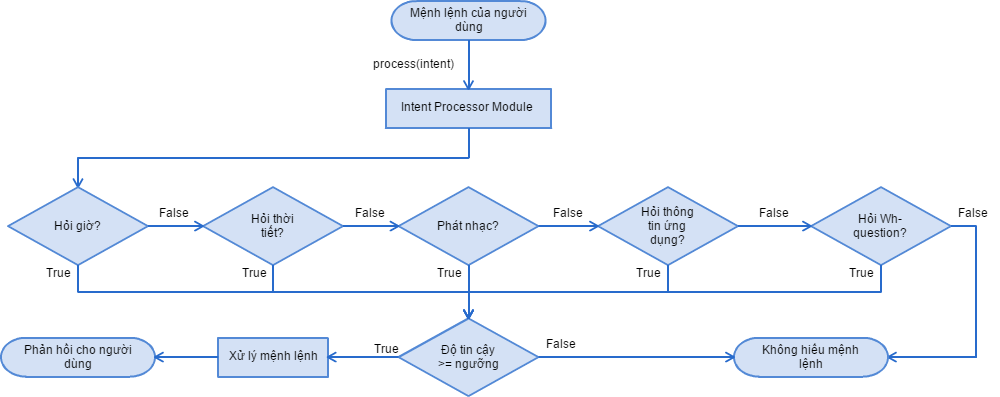
\includegraphics[scale=0.5]{intent_processor_flowchart}
    \caption{Mô hình hoạt động của module Intent Processor}
    \label{fig:c6_intent_processor_flowchart}
\end{figure}

\item \textbf{Cài đặt}: Module Intent Processor được cài đặt theo mẫu Singleton để có thể được sử dụng từ bắt kỳ module nào mà không câng khởi tạo nhiều instance. Trong module Intent Processor sẽ chứa instance của nhiều skill khác nhau. Mỗi skill đảm nhận giải quyết một nhiệm vụ. Khi nhận được yêu cầu người dùng từ module Intent Detector, module Intent Processor sẽ chọn ra skill phù hợp và giao cho nó xử lý yêu cầu người dùng.

Đoạn code xử lý chính của module Intent Processor:
\begin{lstlisting}
class IntentProcessor:
    instance = None

    @staticmethod
    def getInstance(callback = None):
        if IntentProcessor.instance is None:
            IntentProcessor.instance = IntentProcessor(callback)
        return IntentProcessor.instance

    def __init__(self, callback):
        print "Init Intent Processor"
        self.tts = TextToSpeech.getInstance()

        listSkills = [TimeSkill, WeatherSkill, MusicSkill, GeneralQuestionSkill, VolumeSkill, SmalltalkSkill]
        self.skills = {}

        for skill in listSkills:
            self.skills[skill.intent] = skill.getInstance()
        
        self.callback = callback

    def process(self, info):
        try:
            print info['intent']['name'] + ": " + str(info['intent']['confidence'])
            key = info['intent']['name'].split('.')[0]
            if key in self.skills:
                self.skills[key].process(info, self.callback)
            else:
                print "Comming soon"
        except:
            self.tts.play("./Audio/do-not-understand-intent.mp3")

    def getSkill(self, intent):
        if intent in self.skills:
            return self.skills[intent]
        return None

    def addSkill(self, skill):
        self.skills[skill.intent] = skill.getInstance()
\end{lstlisting}

Đoạn code minh họa cách xử lý của một skill:
\begin{lstlisting}
class SmalltalkSkill:
    intent = 'smalltalk'
    name = '...'
    description = "..."
    
    instance = None
    @staticmethod
    def getInstance():
        if SmalltalkSkill.instance is None:
            SmalltalkSkill.instance = SmalltalkSkill()
        return SmalltalkSkill.instance

    def __init__(self):
        self.tts = TextToSpeech.getInstance()
        self.responses_file = "./Response/response-rasa-smalltalk.json"
        self.responses = {}
        self.responseControl = ResponseControl.getInstance()

        with open(self.responses_file, 'r') as f:
            self.responses = json.load(f)
    
    def process(self, intent, callback):
        if intent['intent']['confidence'] < 0.1:
            self.tts.play("./Audio/do-not-understand-intent.mp3")
            return
        
        if intent['intent']['name'] in self.responses:
            responses_text =  self.responses[intent['intent']['name']]
            text = responses_text[random.randint(0, len(responses_text) - 1)]

            if intent['intent']['name'] == "smalltalk.agent.name":
                callback.wakeupModule.onThread(callback.wakeupModule.pause)
                rs.ttsEndCallback = callback.wakeupModule
                rs.ttsEndFunction = callback.wakeupModule.resume
            self.response(text)
        else:
            self.response("uh")

    def response(self, text):
        self.responseControl.textResponse(text)
        self.tts.speak(text)
\end{lstlisting}
\item \textbf{API}: Các hàm tương tác mà module Intent Processor cung cấp
\begin{itemize}
\item \lstinline{process(intent)}: nhận mệnh lệnh người dùng và xử lý.
\item \lstinline{getSkills(intent)}: chọn skill phù hợp để xử lý \lstinline{intent}.
\item \lstinline{addSkills(skill)}: thêm skill vào module.
\end{itemize}
\end{itemize}

\section{Các chức năng chính}

\subsection{Thông báo giờ}

\subsubsection{Chức năng chi tiết:}

Trợ lý ảo có thể cho người dùng biết thời gian tại địa điểm hiện tại của người dùng, hoặc tại một địa điểm bất kỳ nào đó.

\subsubsection{Cách hoạt động:}

\begin{itemize}
    \item Có thể request Google Maps Time Zone API để tìm chênh lệch giờ của một địa điểm so với múi giờ UTC. Tuy nhiên, Time Zone API chỉ nhận địa điểm bằng tọa độ chứ không nhận tên địa điểm. Do đó, hệ thống sẽ phải tìm tọa độ của địa điểm đó.
    \item Nếu trong câu hỏi của người dùng không có địa điểm thì hệ thống sẽ request đến IPInfoDB để tìm tọa độ gần đúng của máy.
    \item Nếu trong câu hỏi có tên địa điểm thì sẽ dùng Google Maps Geocode API để tìm tọa độ của địa điểm đó.
    \item Sau khi tìm được chênh lệch giờ so với UTC, lấy chênh lệch đó cộng với timestamp hiện tại, rồi dùng lớp \lstinline{datetime} của Python để tạo câu trả lời theo format giờ (ví dụ "It's 4:15 PM").
\end{itemize}

\subsection{Thông báo thời tiết}

\subsubsection{Chức năng chi tiết:}

Trợ lý ảo có thể cho người dùng biết thời tiết tại địa điểm hiện tại của người dùng, hoặc tại một địa điểm bất kỳ nào đó.

\subsubsection{Cách hoạt động:}

\begin{itemize}
    \item Nếu trong câu hỏi của người dùng không có địa điểm thì hệ thống sẽ request đến IPInfoDB để tìm địa điểm hiện tại của máy.
    \item Sau khi có tên địa điểm, request đến Apixu API để lấy thông tin thời tiết, sau đó in ra các thông tin đó theo format phù hợp.
\end{itemize}

\subsection{Phát nhạc}

\subsubsection{Chức năng chi tiết:}

Trợ lý ảo có khả năng phát nhạc theo yêu cầu của người dùng (tên bài, tên ca sĩ). Trong lúc phát nhạc có thể tạm dừng, dừng hẳn hoặc sang bài tiếp theo.

\subsubsection{Cách hoạt động:}

Sử dụng Zing MP3 API để tìm bài hát, lưu lại danh sách các bài hát tìm được và stream nhạc từ Zing MP3 về khi biết được ID bài hát.

\subsection{Giao tiếp cơ bản}

\subsubsection{Chức năng chi tiết:}

Trợ lý ảo có thể trả lời một số câu giao tiếp đơn giản như chào, chào buổi sáng, chúc ngủ ngon, hỏi tên, tuổi,...

\subsubsection{Cách hoạt động:}

Trong hệ thống sẽ có danh sách một số câu trả lời cho mỗi intent, khi câu nói của người dùng được phân lớp ra intent nào thì sẽ lấy một câu trả lời ngẫu nhiên trong danh sách câu trả lời của intent đó.

\subsection{Trả lời câu hỏi Wh-question}

\subsubsection{Chức năng chi tiết:}

Trợ lý ảo có khả năng trả lời một số câu hỏi WH-question đơn giản (what, when, who, where, which, how).

\subsubsection{Cách hoạt động:}

Khi nhận được câu hỏi, hệ thống sẽ dùng câu hỏi đó để request đến WolframAlpha Spoken Result API để lấy câu trả lời.

\section{Giao diện hoạt động của ứng dụng}

\begin{figure}[h]
    \centering
    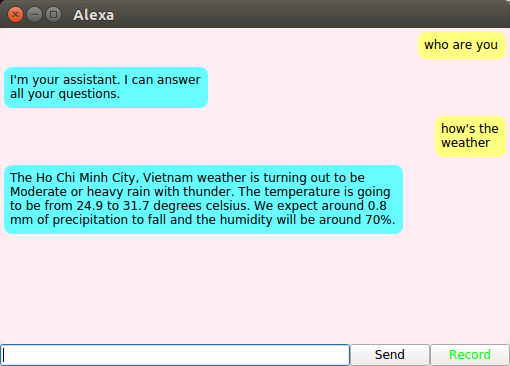
\includegraphics[scale=0.7]{interface}
    \caption{Giao diện hoạt động của ứng dụng Alexa}
    \label{fig:c6_interface}
\end{figure}

Ứng dụng cho phép người dùng ra lệnh bằng một trong hai cách: gõ lệnh vào khung input hoặc ra lệnh bằng lời nói (gọi tên "Alexa" trước khi ra lệnh). Ứng dụng sẽ phản hồi cho người dùng dưới dạng lời nói và văn bản.
